\documentclass{article} % For LaTeX2e
\usepackage{neurips,times}
\usepackage{hyperref}
\usepackage{url}
\usepackage{booktabs}       % professional-quality tables
\usepackage{graphicx}
\usepackage{lipsum}
\usepackage{amsmath}
\usepackage{multirow}

\usepackage[utf8]{inputenc} % allow utf-8 input
\usepackage[T1]{fontenc}    % use 8-bit T1 fonts
\usepackage{hyperref}       % hyperlinks
\usepackage{url}            % simple URL typesetting
\usepackage{booktabs}       % professional-quality tables
\usepackage{amsfonts}       % blackboard math symbols
\usepackage{nicefrac}       % compact symbols for 1/2, etc.
\usepackage{microtype}      % microtypography
\usepackage{amssymb,amsmath,bm}
\usepackage{color,soul}
\usepackage{multirow}
\usepackage{mathtools}


\usepackage[numbers]{natbib}
\setlength{\bibsep}{0.0pt}

\title{Unsupervised Learning of Disentangled and Interpretable Representations from Sequential Data\\ \vspace{0.5cm}\large{Report}}
\author{Stefan Wezel \\ stefan.wezel@student.uni-tuebingen.de \\4080589  \\ ML4S}

\newcommand{\fix}{\marginpar{FIX}}
\newcommand{\new}{\marginpar{NEW}}

\nipsfinalcopy

\begin{document}


\maketitle

\begin{abstract}
%Sequential data often has the intrinsic quality of containing information playing out on multiple time scales. Features can appear low frequencies and on high frequencies. 

%
%While Variational Autoencoders (VAE) have proven to be a successful methodology on i.e. image data, 



Information in sequential data is often distributed over multiple time scales.
While if viewed as a single signal, such data might appear noisy. However, patterns can emerge if temporal scales are viewed separately from one another.
\citet{hsu2017unsupervised} leverage this intrinsic structure to learn disentangled representations from sequential data in an unsupervised manner with a proposed factorized hierarchical variational autoencoder (FHVAE). They aim to factorize sequence level and segment level attributes into distinct latent subspaces. Architectural and sequence dependent priors create an inductive bias to encourage the proposed factorization. Here, we put their work into a formal context, explore the proposed methodology, and reflect critically on their work.
\end{abstract}

\section*{Introduction}
%Learning disentangled representations has long been a difficult problem in machine learning. 
Intuitively, disentangled representations are reflective of the underlying generating factors of observed data in thus they are encoded as separate latent subspaces. This notion is already present in classical factor analysis work, where it is referred to as independent component analysis (ICA) \cite{comon1992independent}.\\
However, many problems cannot be solved in linear fashion. The vast success of deep neural networks (DNN) can be largely attributed to the fact that they are very powerful non-linear function approximators. Thus, making them an promising method to solve the long standing problem of non-linear ICA.\\
Different methods have been proposed to learn such disentangled representations \cite{higgins2016beta, chen2016infogan, kulkarni2015deep} with varying success. Many of these works focus on image data. However, it has been shown by \citet{locatello2019challenging} that disentangled representations cannot by learned without introducing any kind of supervision or inductive biases. Sequential data, while having been explored less, despite offers inherent structure that can be exploited to construct inductive biases as has been proposed by \citet{hsu2017unsupervised}.\\
Besides technical challenges, this strain of research suffers from the lack of formally defined and agreed upon foundations. The very term of disentangled representations for example is often understood differently in between works. In the following section, we will use the definition, proposed by \citet{higgins2018towards} to put the work by \citet{hsu2017unsupervised} into formal context. 

%It would provide a remedy to problems such as uninterpretable representation.
\begin{figure}
	\centering
	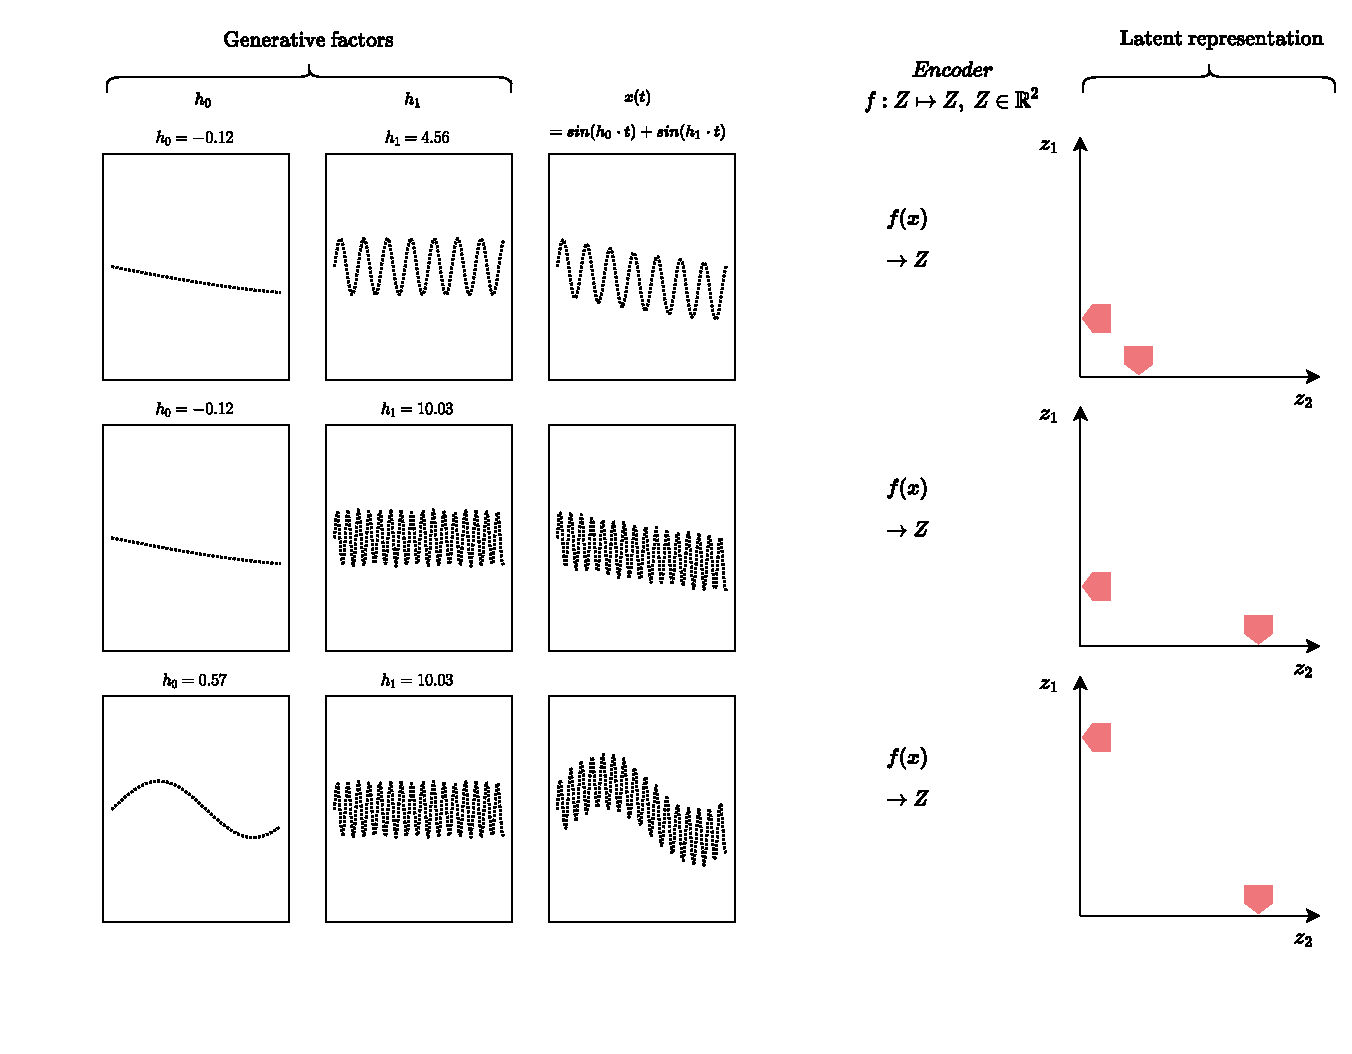
\includegraphics[width=.6\linewidth]{../figures/intution_3x3_static.pdf}
	\caption{Changing values of generating factors are reflected in the corresponding latent variables.}
\end{figure}
%It would provide a remedy to problems such as uninterpretable representation.

%Since \citet{locatello2019challenging} proved that learning such representations without any supervision or inductive biases is impossible, many works have focused on 

%\lipsum[2-3] (Figure \ref{fig:figure_01}).

%\begin{figure}[h]
%    \includegraphics[width=\textwidth]{figures/figure1.png}
%    \caption{kjsdflkajsdkfjsd}
%    \label{fig:figure_01}
%\end{figure}

\section*{Viewing the FHVAE though a Formal Lense}
%\lipsum[4-6]\cite{Papamakarios2016, Ardizzone2019}
Works on disentanglement often lack a proper formal framework \cite{higgins2018towards}. While claiming to achieve disentanglement, \citet{hsu2017unsupervised} do not provide any formal foundation for their claim. With no formal tools at hand, we cannot formally discuss whether disentanglement was achieved. Thus, we use the following sections to respectively give a theoretical background that defines disentanglement in group theoretic terms, and describe the problem, the FHVAE was designed to solve, in these terms.

\subsection*{The Tools of Group Theory}
A group is described by a tuple of an operation $\circ$ and a non-empty set $G$. The set has to be closed under the operation, it must contain an identity element, the operation must be associative, and for every element in $G$, there must be an inverse element \cite{benkart1987abstract}.
%TODO direct product
Multiple groups $G_i$ can be combined via a direct product $G = G_1 \times ... \times G_n$. The result of this direct product is itself a group.\\%, where operations $\circ_{G_i}$ act each respective sets $G_{G_i}$ of each subgroup.
A group that is of particular interest for the field of disentangled representation learning is the symmetry group \cite{benkart1987abstract}.
A symmetry group consists of a set of transformations that leave a given object $X$ invariant and the operation is the composition of such transformations. A prominent example of a symmetry group is $SE_3$. This symmetry group can be visualized as a set set of vertices $X$ that form an equilateral triangle. Permutations of this set would result in rotations or flips of the triangle. These permutations would be the symmetry transformations of our symmetry group. The operation would be composing multiple permutations.\\
Another important concept is the group action. It is the result of applying a symmetry transformation to an object. In our triangle example, a group action would be the permuted set of vertices.\\
If a group action on $X$ is the result of a subset $G_i$ of symmetries $G= G_1 \times ... \times G_n$ and only affects a subset $X_i$ of $X$ but leaves all other $X_{j\neq i}$ unchanged, we say it is a disentangled group action. Now, such disentangled group actions are of particular interest for disentangled representation learning, and are generally what we want to model. Note, that if we observe such disentangled group actions, we can infer that $G$ can be decomposed into a direct product of symmetry groups $G_i$ without knowing the underlying processes.\\
To model such a process, we need to find some symmetry preserving mapping $f:X\mapsto Z$. It should not matter, whether $X$ is mapped to $Z$ followed by applying a symmetry $G$ or $G$ is applied to $X$ and then mapped to $Z$. The resulting space $Z$ should be the same. This is visualized below.
\begin{align*}
%\begin{align}
&X \;\xrightarrow[\text{}]{G}\;\;X\\ 
f&\downarrow \;\;\;\;\;\;\;f\downarrow\\
&Z \;\xrightarrow[\text{}]{G}\;\;\;Z
\end{align*}
Such a mapping is called an equivariant map and its result is a disentangled representation. The space $Z$ (which we will refer to as latent space in the following) naturally decomposes into a direct product of independent subspaces $Z_1 \times ... \times Z_n$. Moreover, each subspace $Z_i$ is only affected by symmetry $G_i$ on $X$ (as only $X_i$ is changed) and remains invariant to all other $G_{j \neq i}$.\\
Note that it is only disentangled with respect to a certain decomposition. This is important, as it means we can only discuss whether disentanglement was achieved, if the decomposition is sufficiently clear. Not all decompositions make sense or are possible to model.\\
As these concepts are rather abstract, we will use the next section to frame the real-world setting of \citet{hsu2017unsupervised} using group theoretic terms to build further intuition and build a formal foundation to discuss their work.


\subsection*{Symmetries in Sequential Data}
\citet{hsu2017unsupervised} argue that certain sequential data can be factorized into attributes of different temporal scale. For example, voice recordings can be decomposed into sequence attributes and segment attributes. In this context, sequence attributes are features that remain unchanged over multiple sequences if spoken by the same speaker. Segment attributes on the other hand, vary in(-between?) sequences and are independent from the speaker. They are determined by variables such as linguistic content.\\
In group theoretic terms, we could state this as the group $G$ acting on audio recordings $X$ is a direct product of $G_{sequence} \times G_{segment}$, because we observe the resulting disentangled group actions of this decomposition. \citet{hsu2017unsupervised} now want to find a representation that is disentangled with respect to this decomposition. They need to find an equivariant map $f:X\mapsto Z$, where $Z = (z_1, z_2)$ is a latent space, so that i.e. $z_2$ is only affected by $G_{sequence}$ and $z_1$ only is affected by $G_{segment}$. Then, the proposed decomposition of symmetries is reflected in $Z$.\\
For this specific setting, finding such an equivariant map, would allow to separate speaker information from content information. This in turn would enable us to reconstruct given content information using another speaker's voice information. \citet{hsu2017unsupervised} propose this as qualitative assessment of their disentanglement. Quantitative evaluation of disentanglement are notoriously challenging and various metrics have been proposed by an active field of research \cite{locatello2019challenging, higgins2016beta}.



\section*{FHVAE - Constructing an Equivariant Map}
\begin{figure}
	\label{fig:fhave}
	\centering
	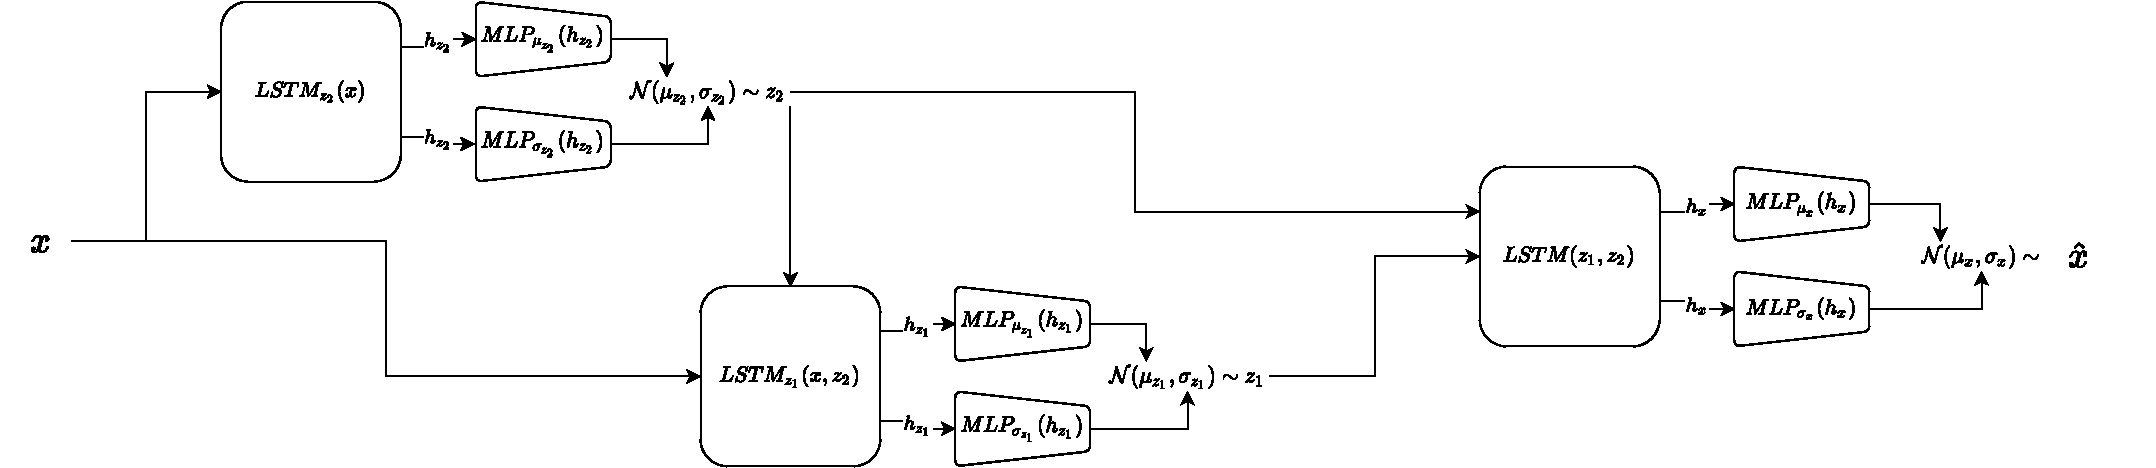
\includegraphics[width=1\linewidth]{../figures/fhvae_complete.pdf}
	\caption{Architecture of the proposed FHVAE. Latent segment variable $z_2$ is conditioned on latent sequence variable $z_1$. Together, they are decoded to form distribution over a reconstructed input $\hat{x}$.}
\end{figure} 
To find an equivariant map for the sequential data setting, \citet{hsu2017unsupervised} porpose the FHVAE (see Figure~\ref{fig:fhave}). They propose a latent subspace factorized into a latent sequence variable $z_1$ and a latent segment variable $z_2$. To form Gaussian distributions over these latent variable, \citet{hsu2017unsupervised} pass an input sequence $x$ to two distinct Long short-term Memory (LSTM) \cite{hochreiter1997long} cells $LSTM_{z_1}$ and $LSTM_{z_2}$. The hidden states of those cells are decoded by Multi-layer Perceptrons (MLP) to give the mean and standard deviation for each latent variable. To decode the latent space, a sample is drawn and passed to another LSTM. This LSTMs hidden state is decoded to form a normal distribution over a reconstructed input $\hat{x}$.\\
To train the FHVAE \citet{hsu2017unsupervised} propose a a segment variational lower bound, similar to \citet{kingma2013auto} and add a discriminative objective.
%\begin{align*}
%\mathcal{L}(\theta, \phi, X)& = \sum_{n=1}^N \underbrace{\mathcal{L}(\theta, \phi;x^{(n)}|\mu_2) + log\;p_{\theta}(\mu_2)+ const.}_{\text{var. lower bound}} + \underbrace{\alpha \cdot log\;(i|z_2^{(i,n)})}_{\text{discrim.obj.}}\\
%\end{align*}
This segment variational lower bound can be written as
\begin{align*}
\mathcal{L}(\theta, \phi, X)& = %\sum_{n=1}^N \mathcal{L}(\theta, \phi;x^{(n)}|\tilde{\mu_2}) + log\;p_{\theta} + const.\\
%\mathcal{L}(\theta, \phi;x^{(n)}|\tilde{\mu_2}) &= 
\underbrace{log\;p(x|z_1, z_2)}_{\text{reconstruction}}\\%prob. of obs. data under learned posterior\\
-&\underbrace{D_{KL}(\mathcal{N}(\mu_{z_1}, \sigma_{z_1})||\mathcal{N}(0,1))}_{\text{regularize $z_1$ with global prior}}\\
-&\underbrace{D_{KL}(\mathcal{N}(\mu_{z_2}, \sigma_{z_2})||\mathcal{N}(\mu_2,0.5))}_{\text{regularize $z_2$ with seq. dep. prior $\mu_2$}}\\
+&\underbrace{log\;p(\mu_2) \cdot \frac{1}{seq.\;length}}_{\text{prob. of $\mu_2$ under standard Gaussian prior}}, 
\end{align*}
where $\theta$ is the set of decoder parameters, $\phi$ are encoder parameters, and $X$ is a dataset. Note that while $z_1$ gets regularized through a standard Gaussian prior, $z_2$ is discouraged to deviate from a Gaussian distribution centered ad $\mu_2$. \citet{hsu2017unsupervised} introduce $\mu_{2}^{(i)}$ as sequence $(i)$-dependent prior to encourage factorization. This sequence dependent prior can be retrieved through a differentiable lookup table. The discriminative objective 
\begin{align*}
log\;p(sequence\;id^{(i)} | z_2^{(i,n)})& = log\;\frac{p(\mu_{z_2}^{(i,n)}|\mu_2^{(i)})}{\sum^{n}_{j=1}	p(\mu_{z_2}^{(i,n)}|\mu_2^{(j)})}
\end{align*}
is used to build an expressive lookup table, where similarity of sequences is reflected by $\mu_{2}^{(i)}$ close in euclidean space.\\
\citet{hsu2017unsupervised} refer to the resulting objective
\begin{align*}
\mathcal{L}^{dis}(\theta, \phi;x)& = \mathcal{L}(\theta, \phi, X) + \alpha \cdot log\;p(sequence\;id | z_2)
\end{align*}
as discriminative segment variational lower bound, where hyperparameter $\alpha$ determines the weight of the discriminative objective.




\section*{Discussion and Future Work}
\citet{hsu2017unsupervised} evaluate the FHVAE on different tasks. They propose an unsupervised speaker verification task to measure performance quantitatively, and to some extent, qualitatively assess the grade of disentanglement. They outperform an i-vector baseline \footnote{According to \citet{hsu2017unsupervised}, i-vector is used in state-of-the-art speaker verification approaches. It is a low dimensional subspace of a Gaussian mixture universal background model which ideally only contains speaker information.}. To identify speakers, they use $\mu_2$ which ideally should only encode speaker dependent attributes. As a sanity check, they further introduce a segment vector $\mu_1$, which is based on $z_1$ and should thus ideally only contain information independent from the speaker. The results are displayed below in Table~\ref{tab:eer}.


\begin{table}[tbh]
	\caption{Comparison of speaker verification equal error rate (EER) on the TIMIT test set.}
	\label{tab:eer}
	\centering
	\begin{tabular}{llll}
		\toprule
		Method 				& Dimension 	& $\alpha$ 		& EER  				 \\
		\midrule\midrule
		\multirow{1}{*}{i-vector}
		& 100   & -     & 9.52\%    \\
		\midrule
		\multirow{1}{*}{$\bm{\mu}_2$}  	& 32			& $10^1$	& \textbf{2.38\%}  	 	\\
		\midrule
		\multirow{1}{*}{$\bm{\mu}_1$}
	& 32			& $10^1$		& 22.47\%   	\\
		\bottomrule
	\end{tabular}
\end{table}
While using $\mu_2$ results in the lowest EER, they still achieve below random-baseline EER using $\mu_1$, indicating leakage of sequence level information into $z_1$.\\
This observation reveals a larger problem. While \citet{hsu2017unsupervised} provide visual and audio qualitative examples to demonstrate the grade of disentaglement, they fail in providing sufficient quantitative evidence.\\
Moreover, their work lacks a formal description and justification of the proposed factorization. We use this work, to 
We propose to further exploit the used data by introducing a cross-reconstruction loss.
%TODO elaborate more on this
 Additionally, we hypothesize that using a hierarchical activation function, as proposed by \citet{shen2018ordered} could further encourage a clean factorization.



%Moreover, their work lacks formal context, in terms of disentanglement.
%\citet{hsu2017unsupervised} evaluate the FHVAE on other tasks, such as automatic speech recognition as well and achieve good results.
%
%
%
%In this work, however, we want to focus on the lack of established formal context.
%
%
%
%Lack of formal context.
%Lack of evidence for disentaglement.
%Further exploit the available data using cross reconstruction.

\section*{Conclusion}
\citet{hsu2017unsupervised} propose an architecture suited to approximate an equivariant map with respect to a sequence-segment decomposition. They exploit the hierarchical nature of certain sequential data to form an inductive bias towards factorization of different temporal scales. We hypothesize that the notion of a sequence dependent prior could be transferred to other settings. While achieving good performance on considered benchmark task, their work lacks quantitative evidence of achieved disentanglement.
%Performance on benchmark tasks is not bad.

We advocate for the need of more foundational, formal work on disentanglement. We hypothesize that this would allow to fairly discuss, evaluate and compare methods. The field might be ahead of itself. 


\newpage
\bibliographystyle{unsrtnat}
\bibliography{refs}

\end{document}
